\section{Entwurfsphase}

\subsection{Architekturdesign}

Als passendes Entwurfsmuster für den Shortcut Editor hat sich das Model View Presenter (MVP)-Architekturmuster herausgestellt. Dieses ist nicht ganz so verbreitet wie das bekanntere Model View Controller (MVC)-Muster, ist diesem aber sehr ähnlich. Der eigendliche Unterschied zwischen MVP und MVC liegt darin, dass bei MVC die View neben dem Controller auch mit dem Model kommuniziert und dieses somit kennen muss. Bei MVP ist die View völlig unabhängig vom Model und nur der Presenter kommuniziert mit ihr (siehe \autoref{fig:modelview}). Der Autor hat sich für das MVP-Entwurfsmuster entschieden, da damit die View auch ohne Model verwendet werden kann und es denkbar ist, das diese Möglichkeit in Zukunft benötigt wird.

\begin{figure}[H] 
	\subfloat{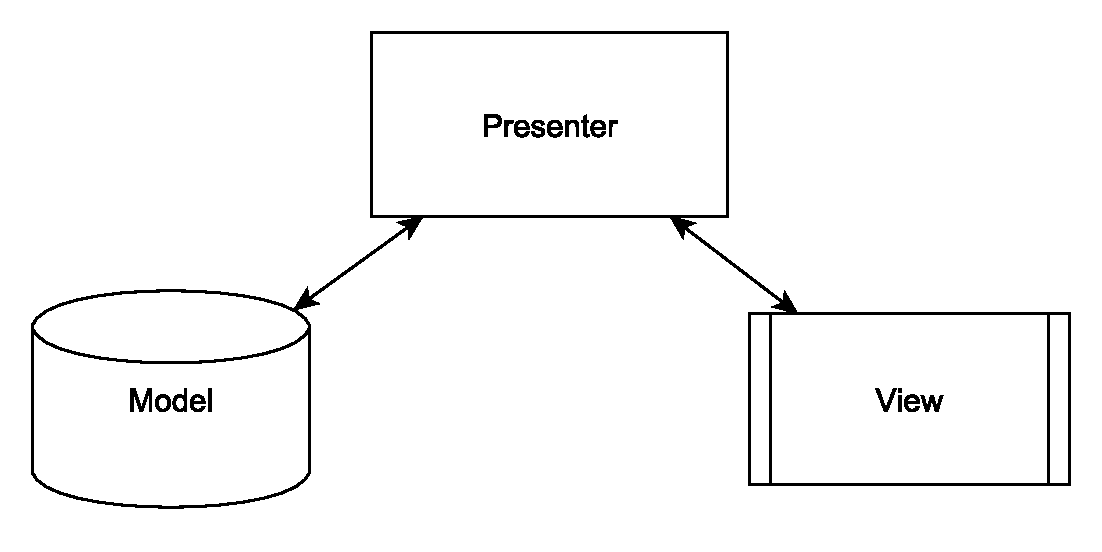
\includegraphics[width=0.5\textwidth-5px]{../img/diagram/ModelViewPresenter/ModelViewPresenter}}
	\hfill 
	\subfloat{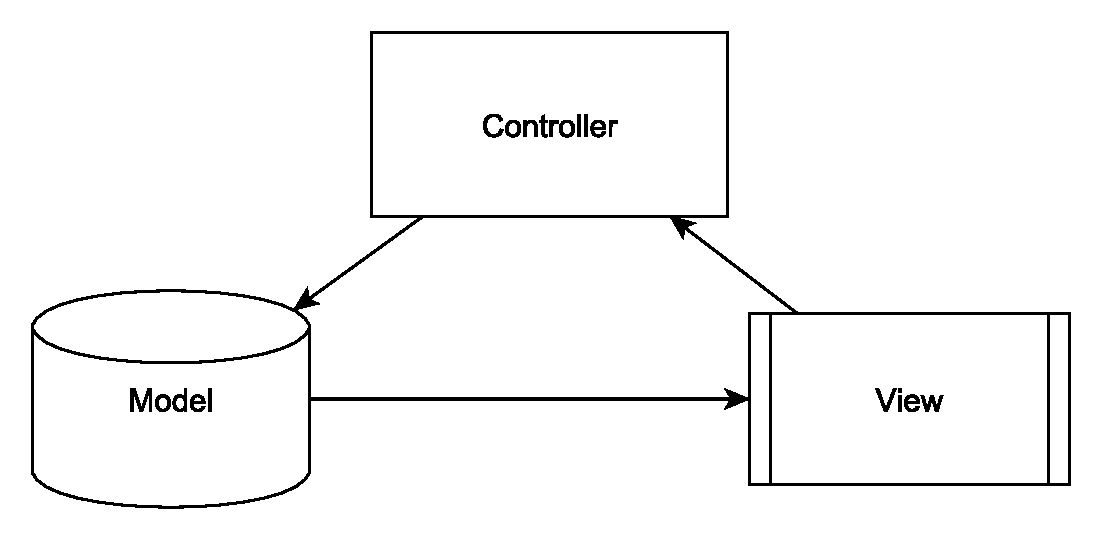
\includegraphics[width=0.5\textwidth-5px]{../img/diagram/ModelViewController/ModelViewController}}
	\caption{Model View Presenter vs. Model View Controller} 
	\label{fig:modelview}
\end{figure}

Bei MVP lässt sich jede Komponente der Software einen der drei Bestandteile - Model, View oder Presenter - zuordnen. Jeder dieser Teile hat einen eigenen Aufgabenbereich, der von denen der Anderen weitestgehend unabhängig ist. Im Model werden alle Daten gehalten und zur Verfügung gestellt. Die View kümmert sich um die grafische Darstellung und der Presenter stellt das Bindeglied zwischen der View und dem Model dar. Verändern sich beispielsweiße die Werte in der View, so kümmert sich der Presenter darum, dass diese Wertänderung im Model ebenso stattfindet und andersherum. Der Presenter hält somit die View -- oder auch mehrere Views untereinander -- und das Model synchron zueinander. Die lose Kopplung der einzelnen Komponenten erhöht die Wiederverwendbarkeit und Austauschbarkeit. Man könnte beispielsweise die Benutzeroberfläche austauschen, ohne das Model anpassen zu müssen. Außerdem können die einzelnen Komponenten durch die strikte Trennung einfacher getestet, gewartet und flexibel erweitert werden. Diese Vorteile sprechen ebenso für eine Verwendung von MVP.

Im Sinne der Wiederverwendbarkeit, werden alle GUI-Komponenten des Shortcut Editors völlig seperat voneinander und unabhängig vom Editor implementiert. Dadurch kann gewährleistet werden, keine unnötigen Abhängigkeiten zu Editorspezifischen Teilen aufzubauen. So ist die Benutzung von Komponenten auch an anderen Stellen in der Software ohne weiteren Aufwand möglich.

Wie im Abschnitt \ref{schnittstellen} bereits erwähnt wird für das Lesen der Testergebnis XML-Dateien das hauseigene Propertly Framework verwendet. Dieses Tool stellt Funktionalitäten zum Lesen und Schreiben von XML zur Verfügung. Außerdem kümmert es sich eigendständig um die Konvertierung von Datentypen. Dadurch kommt der Autor bei der Implementierung nicht mit XML spezifischen Arbeiten in Berührung und kann sich auf den eigentlichen Editor konzentrieren.

\newpage

\subsection{Benutzeroberfläche}

Für das Design des User Interfaces wurden von unserem UX-Designer Entwürfe angefertigt (siehe \autoref{fig:uxDesigns}). Im Designentwurf wird ersichtlich, welche Komponenten verwendet werden müssen, um alle angeforderten Informationen darzustellen und die bedarfsgerechte Bedienung zu ermöglichen.

(XXX) Erläuterung

\begin{figure}[H] 
	\subfloat{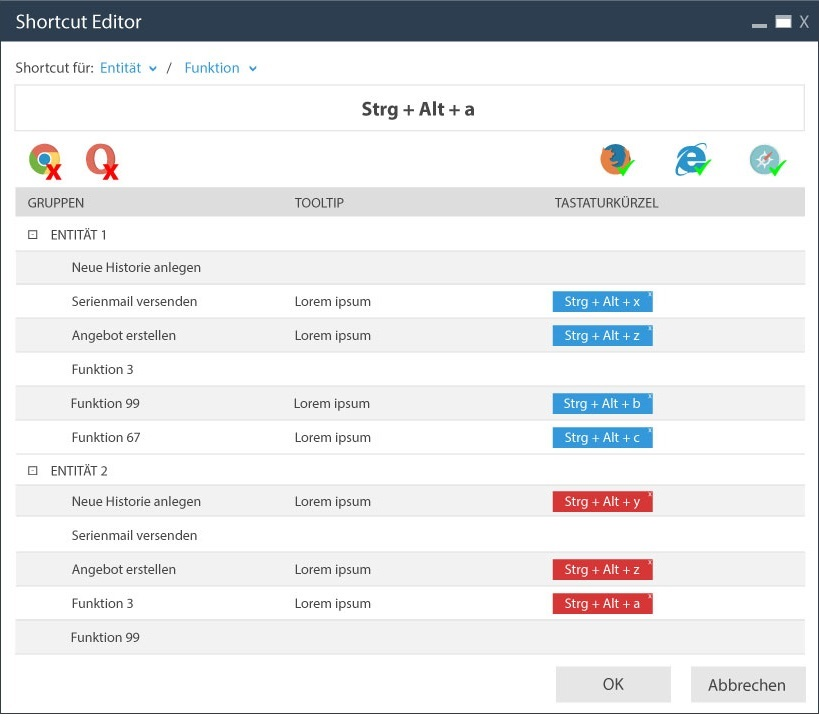
\includegraphics[width=0.5\textwidth-5px]{../img/ux/2-ShortCutEditor-Eingabe.jpg}}
	\hfill 
	\subfloat{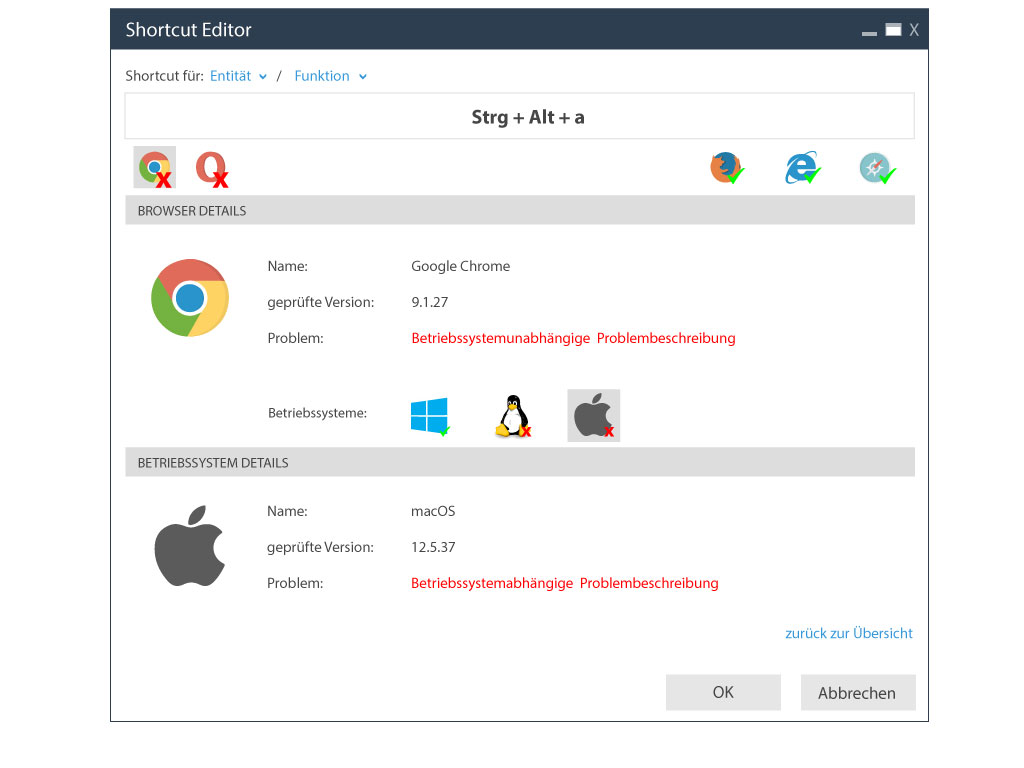
\includegraphics[width=0.5\textwidth-5px]{../img/ux/4-ShortCut-Info.jpg}}
	\caption{UI-Entwürfe der UX Abteilung} 
	\label{fig:uxDesigns}
\end{figure}



\newpage